%\documentclass[aspectratio=43]{beamer}

%
\documentclass[10pt]{beamer}

\usepackage{xeCJK}
\setCJKmainfont{蘋方-繁}

\setbeamertemplate{caption}[numbered] %加入圖片

\usetheme[progressbar=frametitle]{metropolis}
\usepackage{appendixnumberbeamer}
\usepackage{color}

\usepackage{booktabs}
\usepackage[scale=2]{ccicons}

\usepackage{pgfplots}
\usepgfplotslibrary{dateplot}

\usepackage{xspace}
\usepackage{listings}
\newcommand{\themename}{\textbf{\textsc{metropolis}}\xspace}
%

%\usepackage[english]{babel}
%\usepackage{mathtools}
%\usepackage{amsmath}

%\usepackage[backend=biber]{biblatex}

%\usepackage{amsthm}
\usepackage{mathtools}
\usepackage{physics}
\usepackage{calligra}
\usepackage{csquotes}
\usepackage{tensor}
\usepackage[thicklines]{cancel}
\usepackage{tcolorbox}
\usepackage{pstricks}
\usepackage[backend=biber, bibstyle=nature, sorting=nty, citestyle=numeric-comp]{biblatex} %Custom bibliography
    \addbibresource{bib.bib} %Load references


\DeclareMathAlphabet{\mathcalligra}{T1}{calligra}{m}{n}
\DeclareFontShape{T1}{calligra}{m}{n}{<->s*[2.2]callig15}{}
\newcommand{\scriptr}{\mathcalligra{r}\,}
\newcommand{\boldscriptr}{\pmb{\mathcalligra{r}}\,}
\def\rc{\scriptr}
\def\brc{\boldscriptr}
\def\hrc{\hat\brc}
\newcommand{\ie}{\emph{i.e.}} %id est
\newcommand{\eg}{\emph{e.g.}} %exempli gratia
\newcommand{\rtd}[1]{\ensuremath{\left\lfloor #1 \right\rfloor}}
\newcommand{\dirac}[1]{\ensuremath{\delta \left( #1 \right)}}
\newcommand{\diract}[1]{\ensuremath{\delta^3 \left( #1 \right)}}
\newcommand{\e}{\ensuremath{\epsilon_0}}
\newcommand{\m}{\ensuremath{\mu_0}}
\newcommand{\V}{\ensuremath{\mathcal{V}}}
\newcommand{\prnt}[1]{\ensuremath{\left(#1\right)}} %parentheses
\newcommand{\colch}[1]{\ensuremath{\left[#1\right]}} %square brackets
\newcommand{\chave}[1]{\ensuremath{\left\{#1\right\}}}  %curly brackets

\useoutertheme{infolines}
\useinnertheme{rectangles}
\usefonttheme{professionalfonts}


\definecolor{orange}{HTML}{f28165}
\definecolor{gray}{HTML}{303030}
\definecolor{yellow}{HTML}{f0be52}
\definecolor{lightorange}{HTML}{f19e58}

\renewcommand{\CancelColor}{\color{orange}}

\makeatletter
\newcommand{\mybox}[1]{%
  \setbox0=\hbox{#1}%
  \setlength{\@tempdima}{\dimexpr\wd0+13pt}%
  \begin{tcolorbox}[colback=orange,colframe=orange,boxrule=0.5pt,arc=4pt,
      left=6pt,right=6pt,top=6pt,bottom=6pt,boxsep=0pt,width=\@tempdima]
    \textcolor{white}{#1}
  \end{tcolorbox}
}
\makeatother

\usecolortheme[named=orange]{structure}
\usecolortheme{sidebartab}
\usecolortheme{orchid}
\usecolortheme{whale}
\setbeamercolor{alerted text}{fg=yellow}
\setbeamercolor{block title alerted}{bg=alerted text.fg!90!black}
\setbeamercolor{block title example}{bg=lightorange!60!black}
\setbeamercolor{background canvas}{bg=gray}
\setbeamercolor{normal text}{bg=gray,fg=white}

\setbeamertemplate{footline}
        {
      \leavevmode%
      \hbox{%
      \begin{beamercolorbox}[wd=.333333\paperwidth,ht=2.25ex,dp=1ex,center]{author in head/foot}%
        \usebeamerfont{author in head/foot}\insertshortauthor~~(\insertshortinstitute)
      \end{beamercolorbox}%
      \begin{beamercolorbox}[wd=.333333\paperwidth,ht=2.25ex,dp=1ex,center]{title in head/foot}%
        \usebeamerfont{title in head/foot}\insertshorttitle
      \end{beamercolorbox}%
      \begin{beamercolorbox}[wd=.333333\paperwidth,ht=2.25ex,dp=1ex,center]{date in head/foot}%
        \usebeamerfont{date in head/foot}\insertshortdate{}%\hspace*{2em}

    %#turning the next line into a comment, erases the frame numbers
        %\insertframenumber{} / \inserttotalframenumber\hspace*{2ex} 

      \end{beamercolorbox}}%
      \vskip0pt%
    }


\setbeamertemplate{blocks}[rectangle]
\setbeamercovered{dynamic}

\setbeamertemplate{section page}
{
	\begin{centering}
		\begin{beamercolorbox}[sep=27pt,center]{part title}
			\usebeamerfont{section title}\insertsection\par
			\usebeamerfont{subsection title}\insertsubsection\par
		\end{beamercolorbox}
	\end{centering}
}

%\setbeamertemplate{subsection page}
%{
%	\begin{centering}
%		\begin{beamercolorbox}[sep=12pt,center]{part title}
%			\usebeamerfont{subsection title}\insertsubsection\par
%		\end{beamercolorbox}
%	\end{centering}
%}

\newcommand{\hlight}[1]{\colorbox{violet!50}{#1}}
\newcommand{\hlighta}[1]{\colorbox{red!50}{#1}}
\title{如何奪得先機搶發PTT地震爆文?} %->->->->-> Check hyperref title <-<-<-<-<-
\subtitle{2020 Spring ccClub Project}
\author[Boyie]{陳柏瑜、高翊傑、蔡易辰}
\institute[NTU]{
    Graduate Institute of Economics\\
    National Taiwan University\\
} %You can change the Institution if you are from somewhere else
\date{\today}
%\logo{\includegraphics[width= 0.2\textwidth]{images/a-logo.png}}

\begin{document}
    
    \frame{\titlepage}

    \begin{frame}{Brief}
        \tableofcontents
    \end{frame}
    
    \section{Inroduction}
    %\frame{\sectionpage}

%%
\begin{frame}[fragile]{Motivation}

有使用過PTT的人都不陌生,每當地震後第一件要做的事情不是報平安,而是到八卦版上發地震文。

在2020/5/3上午11:29,我在臺大社科院感受到地震,幾秒後我突然好奇,若在這時打開PTT的八卦版,會看到幾篇地震文。結果已然有十數篇,更發現第一篇早已推爆,且發文時間在11:28:18。這意味者早在我感受到地震以前,在別處已有人感受到地震而發文。

這不但受地震的傳播速度影響,更讓我發想了以下的問題:究竟還有哪些因素影響著人們「能夠搶到PTT的地震爆文」呢?

\end{frame}

%%
\begin{frame}[fragile]{問題發想}

根據{\color{blue}\href{http://scimonth.blogspot.com/2009/09/blog-post_1815.html}{科學月刊}}的文章,P波每秒走5-7 km,S波每秒走3-4 km。而5/3上午的地震震央在台東臺北方海域,爆文則由來自台中的網友奪得。上一次在八卦版有文章的地震則是4/12,震央及爆文發文者均在宜蘭。
因此可以提出以下的問題:

- PTT使用者與震央的遠近是否會顯著地影響奪得爆文的機率

與此同時,我們必須進一步問的可能就是,如果會,那麼:

- 如果其他條件不變,我所處的縣市距離震央每遠一公里,會比別人多花幾秒鐘發文?

\end{frame}

%%
\begin{frame}[fragile]{問題發想}

為了要回答這個問題,我們顯然需要發文者的位置,幸好PTT已經紀錄了IP位址,我們只要反查即可。如:{\color{blue}\href{https://www.ez2o.com/App/Net/IP}{反查IP網站}}

以及利用中央氣象局發佈的地震報告當中的震央資訊,即可比對發文者位置與震央位址的遠近。

此外,我們還好奇,是否有「縣市別」的因素影響著PTT使用者是否搶到地震爆文。例如:人口密度、各縣市的平均移動網路速度等。

\end{frame}


%%
\begin{frame}[fragile]{Approach}

我們以如下的方式獲取資料:

\begin{enumerate}
	\item 以Request及BeautifulSoup爬PTT八卦版關鍵字有「地震」的文章
	\item 以Selenium反查IP位址,紀錄經緯度資訊
	\item 以Pandas套件清資料
\end{enumerate}

\end{frame}



    \section{Data}

%%
\begin{frame}[fragile]{DataFrame}
	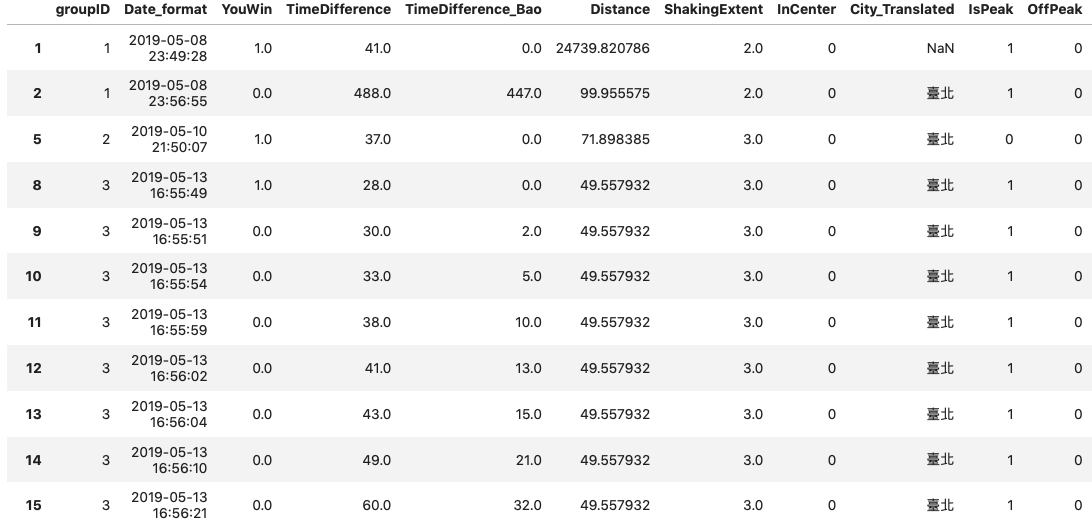
\includegraphics[width=1\textwidth]{Images/data.png}
\end{frame}


%%
\begin{frame}[fragile]{Table of Variables}

\begin{table}[htbp]
\tiny
\begin{tabular}{llll}
Variable            & Description                                      & Type       & 單位     \\
YouWin              & 是否是地震爆文                                          & binary     &        \\
TimeDifference      & 文章發表時間與地震發生時間的時間差                                & continuous & Second \\
TimeDifference\_Bao & 地震文與地震爆文                                         & continuous & second \\
Distance            & 發文者與震央的距離                                        & continuous & km     \\
ShakingExtent       & 震央所在地的震度                                         & level      &        \\
InCenter            & 發文者是否為在震央所在的縣市                                   & binary     &        \\
IsPeak              & 發文者是否在尖峰時段(22:00$\sim$2:00;13:00$\sim$17:00)發文 & binary     &        \\
OffPeak             & 發文者是否在離峰時段(4:00$\sim$8:00; 18:00$\sim$20:00)發文 & binary     &        \\
PopDensity          & 各縣市人口密度                                          & continuous & 人/平方公里 \\
download\_4G        & 各縣市4G移動網路平均下行速率                                  & continuous & Mbps   \\
upload\_4G          & 各縣市4G移動網路平均上行速率                                  & continuous & Mbps  
\end{tabular}

\end{table}
\end{frame}


%%
\begin{frame}[fragile]{About Cleaning Data}

由於由IP位址反查的經緯度僅能定位到「縣市」層級的地理位置,因此與縣市別有關的資料,如:人口密度、4G移動網路下行、上行速率等資料都是以縣市別為單位。

注意到,我們考量的是一場地震的震度,而非規模。因為我們相信震度更能體現體感,即震度能考量到同樣規模下,深、淺層地震給人感受的差別。
又,事實上震度應因縣市而有所不同,然而該資料不易抓取,因此僅納入震央所在地的震度。

\end{frame}

%%
\begin{frame}[fragile]{About Cleaning Data}

尖峰時段與離峰時段的定義方式參考了{\color{blue}\href{https://www.ptt.cc/statistics.html}{PTT Statistics}}的統計數據

將波峰的前後兩小時定義為尖峰時段;將波谷的前後兩小時定義為離峰時段。

	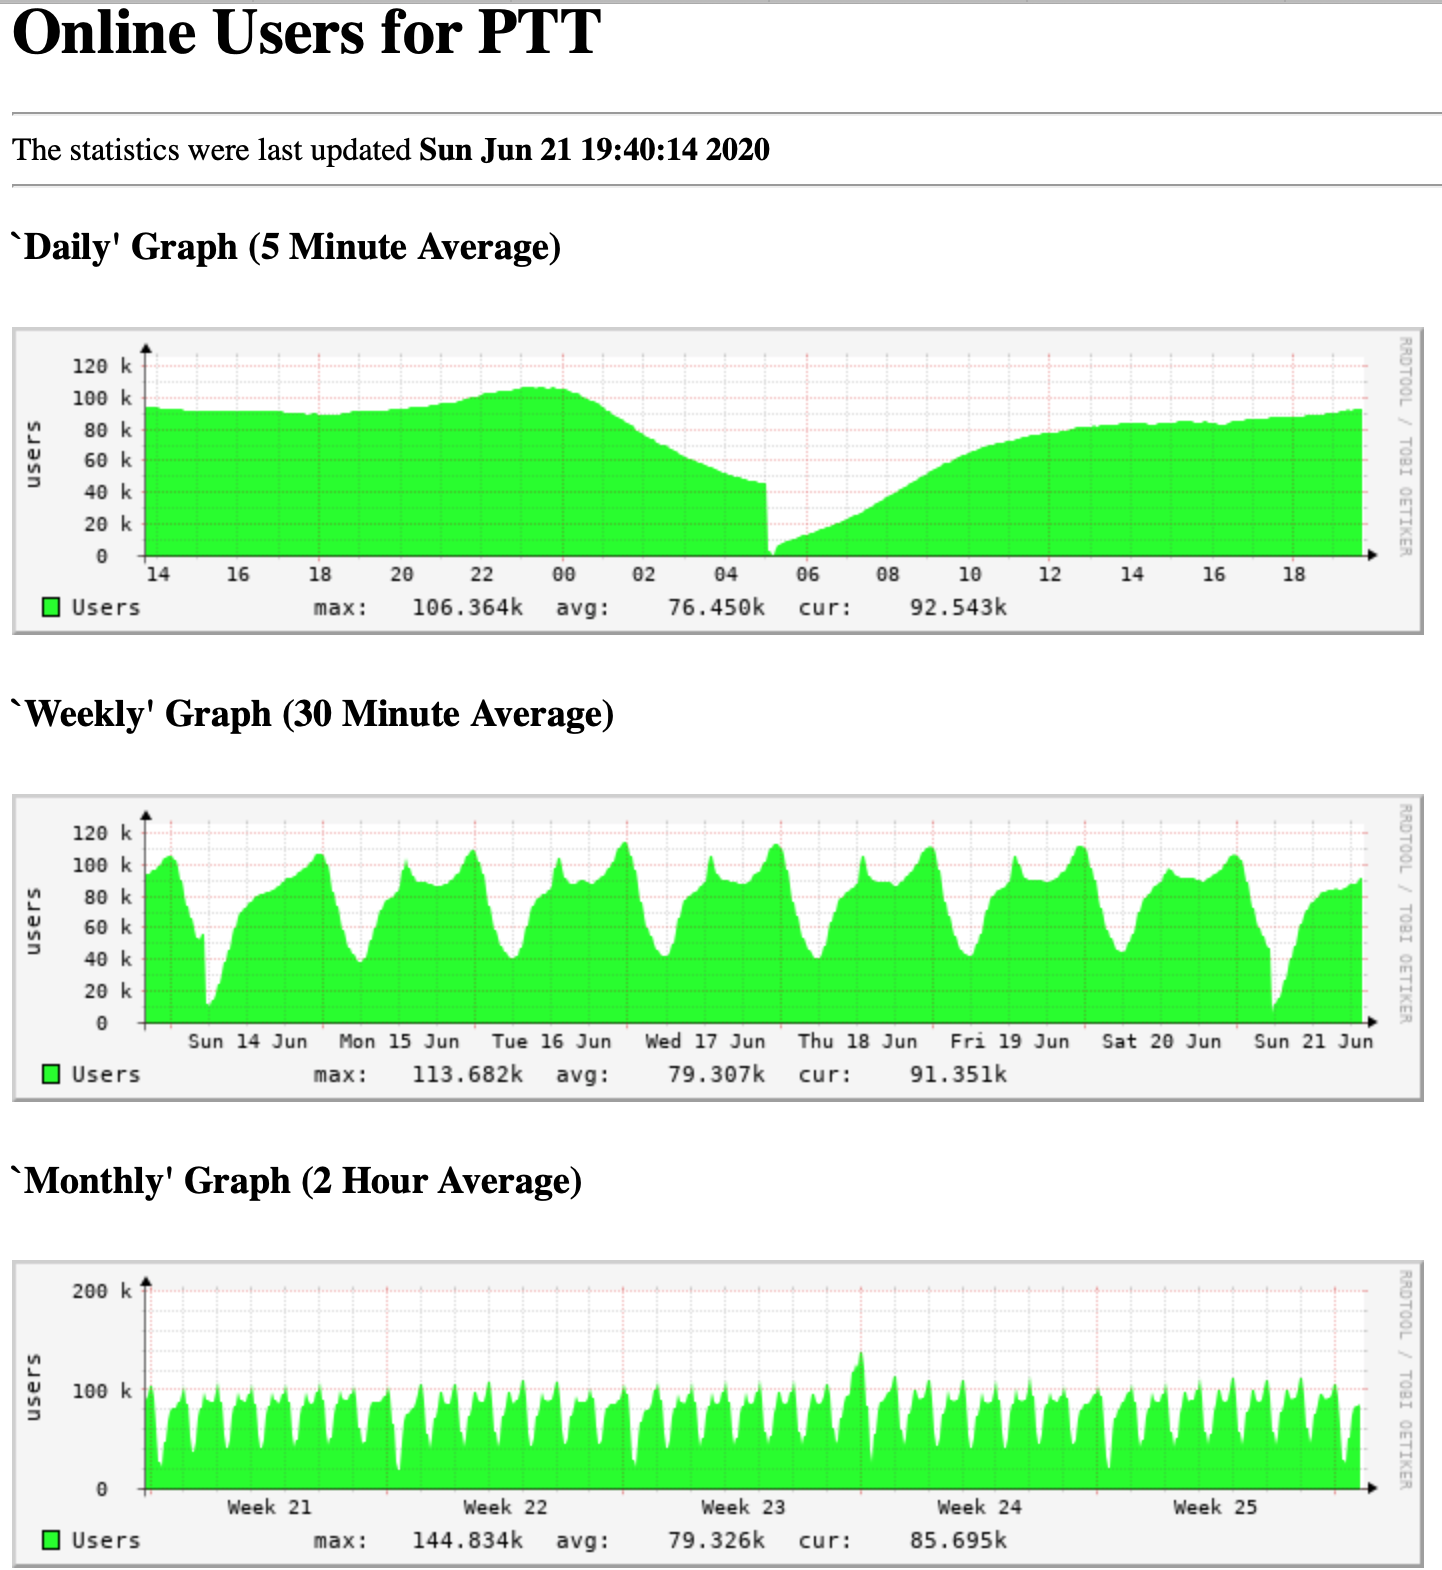
\includegraphics[width=0.5\textwidth]{Images/peak.png}

\end{frame}


%%
\begin{frame}[fragile]{About Cleaning Data}

各縣市的4G移動網路速度來自{\color{blue}\href{https://www.inside.com.tw/article/19538-NCC-4G-speed-report-2019}{NCC發佈的報告}}。

	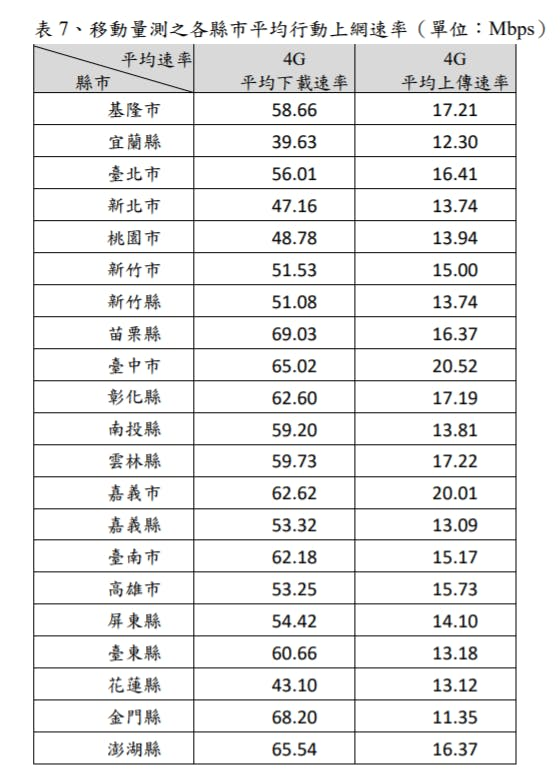
\includegraphics[width=0.5\textwidth]{Images/4g.jpg}

\end{frame}


%%
\begin{frame}[fragile]{About Cleaning Data}

各縣市人口密度資料來自{\color{blue}\href{https://zh.wikipedia.org/wiki/臺灣行政區人口密度表}{Wikipedia}},
由臺灣行政區面積表及臺灣行政區人口列表的資料計算出。

與震央間的距離由經緯度之差{\color{blue}\href{https://wywu.pixnet.net/blog/post/22338038}{簡單換算}}而得:

	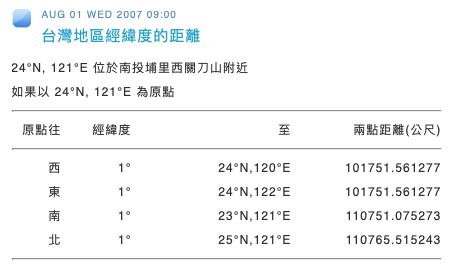
\includegraphics[width=0.7\textwidth]{Images/distance.png}

\end{frame}


    
    

\section{Results}



%%
\begin{frame}[fragile]{Models}

我們分別以\texttt{YouWin}, \texttt{TimeDifference}, \texttt{TimeDifference\_Bao}為被解釋變數。

我們分別以以下三個模型:
\begin{enumerate}
    \item Binary Response
    \item Linear Model
    \item Poisson Regression
\end{enumerate}

來看距離(Distance)對上述被解釋變數的效果為何。

\end{frame}


%%
\begin{frame}[fragile]{Regression Table: Binary Response}

\begin{table}[htbp]
\tiny

\begin{tabular}{lccccc} \hline
 & (1) & (2) & (3) & (4) & (5) \\
VARIABLES & LPM:POLS & LPM:RE & LPM:FE & Probit & Logit \\ \hline
 &  &  &  &  &  \\
distance & -0.00124*** & -0.000957*** & -0.000296 & -0.00416*** & -0.00728*** \\
 & (0.000407) & (0.000348) & (0.000500) & (0.00150) & (0.00275) \\
shakingextent & 0.0195 & -0.00609 &  & 0.0645 & 0.104 \\
 & (0.0397) & (0.0391) &  & (0.124) & (0.218) \\
incenter & 0.00297 & 0.102 & 0.201 & -0.0450 & -0.0844 \\
 & (0.177) & (0.168) & (0.205) & (0.502) & (0.777) \\
ispeak & -0.0732 & -0.0434 &  & -0.209 & -0.360 \\
 & (0.107) & (0.0753) &  & (0.314) & (0.516) \\
offpeak & -0.183* & -0.218** &  & -0.640** & -1.100** \\
 & (0.0955) & (0.0890) &  & (0.297) & (0.484) \\
popdensity & -2.81e-05*** & -1.85e-05** & -1.40e-05* & -8.48e-05*** & -0.000145*** \\
 & (8.49e-06) & (7.45e-06) & (7.23e-06) & (2.51e-05) & (4.20e-05) \\
download\_4g & -0.0141 & -0.0136 & -0.0184 & -0.0420 & -0.0693 \\
 & (0.0113) & (0.0110) & (0.0162) & (0.0330) & (0.0540) \\
upload\_4g & 0.0343 & 0.0396 & 0.0483 & 0.111 & 0.189 \\
 & (0.0286) & (0.0277) & (0.0373) & (0.0821) & (0.137) \\
Constant & 0.847* & 0.872* & 0.619 & 0.957 & 1.555 \\
 & (0.508) & (0.472) & (0.528) & (1.470) & (2.309) \\
 &  &  &  &  &  \\
Observations & 336 & 336 & 336 & 336 & 336 \\
R-squared & 0.143 &  & 0.096 &  &  \\
 Number of groupid &  & 87 & 87 &  &  \\ \hline
\multicolumn{6}{c}{ Robust standard errors in parentheses} \\
\multicolumn{6}{c}{ *** p$<$0.01, ** p$<$0.05, * p$<$0.1} \\
\end{tabular}


\end{table}
\end{frame}


%%
\begin{frame}[fragile]{APE for Probit}

\lstdefinestyle{myCustomMatlabStyle}{
  language=Matlab,
  numbers=left,
  stepnumber=1,
  numbersep=10pt,
  tabsize=7,
  showspaces=false,
  showstringspaces=false
}

% A "tiny" listing
\lstset{basicstyle=\tiny,style=myCustomMatlabStyle}
\begin{lstlisting}
Marginal effects after probit
      y  = Pr(youwin) (predict)
         =  .25759779
------------------------------------------------------------------------------
variable |      dy/dx    Std. Err.     z    P>|z|  [    95% C.I.   ]      X
---------+--------------------------------------------------------------------
distance |  -.0013423      .00047   -2.83   0.005  -.002273 -.000412   103.467
shakin~t |   .0208306      .03972    0.52   0.600   -.05702  .098681   3.11012
incenter*|  -.0143652       .1585   -0.09   0.928  -.325023  .296293   .136905
  ispeak*|  -.0659249      .09777   -0.67   0.500  -.257548  .125698   .357143
 offpeak*|  -.1906436      .08894   -2.14   0.032  -.364967  -.01632    .33631
popden~y |  -.0000274      .00001   -3.61   0.000  -.000042 -.000013   6288.73
downl~4g |  -.0135642      .01079   -1.26   0.209  -.034709   .00758   56.3185
uploa~4g |   .0358601      .02718    1.32   0.187   -.01742   .08914   16.3576
------------------------------------------------------------------------------
(*) dy/dx is for discrete change of dummy variable from 0 to 1

\end{lstlisting}
\end{frame}

%%
\begin{frame}[fragile]{APE for Logit}

\lstdefinestyle{myCustomMatlabStyle}{
  language=Matlab,
  numbers=left,
  stepnumber=1,
  numbersep=10pt,
  tabsize=7,
  showspaces=false,
  showstringspaces=false
}

% A "tiny" listing
\lstset{basicstyle=\tiny,style=myCustomMatlabStyle}

\begin{lstlisting}
Marginal effects after logit
      y  = Pr(youwin) (predict)
         =  .24935992
------------------------------------------------------------------------------
variable |      dy/dx    Std. Err.     z    P>|z|  [    95% C.I.   ]      X
---------+--------------------------------------------------------------------
distance |   -.001363      .00049   -2.80   0.005  -.002318 -.000408   103.467
shakin~t |   .0195255      .04058    0.48   0.630  -.060004  .099055   3.11012
incenter*|  -.0155464      .14083   -0.11   0.912  -.291576  .260483   .136905
  ispeak*|  -.0655836      .09196   -0.71   0.476  -.245821  .114653   .357143
 offpeak*|  -.1867486      .08456   -2.21   0.027  -.352486 -.021012    .33631
popden~y |  -.0000271      .00001   -3.84   0.000  -.000041 -.000013   6288.73
downl~4g |  -.0129651      .01029   -1.26   0.208  -.033138  .007208   56.3185
uploa~4g |   .0354114      .02653    1.33   0.182  -.016588  .087411   16.3576
------------------------------------------------------------------------------
(*) dy/dx is for discrete change of dummy variable from 0 to 1

\end{lstlisting}
\end{frame}

%%
\begin{frame}[fragile]{Interpretations: Binary Response}

在控制住個別縣市的因素後,我們能發現距離(Distance)在絕大部分的模型都能影響「搶到爆文」的機率。

然而其效果大約為:\texttt{在其他條件不變下,每離震央遠一公里,搶到爆文的機率就下降0.13\%}

值得一提的是:一縣市人口密度越高,可能表示網路使用者之間的競爭越激烈,因此與搶到爆文的機率有負向關係。然而人口密度(Density)是控制變數,並非variable of interest,我們暫且不討論其可能存在內生性的問題。

\end{frame}


%%
\begin{frame}[fragile]{Regression Table: TimeDifference}

\begin{table}[htbp]
\tiny

\begin{tabular}{lcccc} \hline
 & (1) & (2) & (3) & (4) \\
VARIABLES & POLS & RE & FE & Poisson \\ \hline
 &  &  &  &  \\
distance & 0.495*** & 0.495*** & 0.267 & 0.00361*** \\
 & (0.133) & (0.133) & (0.230) & (0.000844) \\
shakingextent & 8.619 & 8.619 &  & 0.0614 \\
 & (9.050) & (9.050) &  & (0.0685) \\
incenter & 31.71 & 31.71 & -8.303 & 0.215 \\
 & (24.31) & (24.31) & (52.53) & (0.218) \\
ispeak & -1.807 & -1.807 &  & 0.00103 \\
 & (24.67) & (24.67) &  & (0.196) \\
offpeak & -22.71 & -22.71 &  & -0.155 \\
 & (21.82) & (21.82) &  & (0.171) \\
popdensity & 0.00612*** & 0.00612*** & 0.00326 & 5.38e-05*** \\
 & (0.00185) & (0.00185) & (0.00276) & (1.58e-05) \\
download\_4g & 2.380 & 2.380 & 1.788 & 0.0230 \\
 & (1.766) & (1.766) & (3.341) & (0.0158) \\
upload\_4g & -4.095 & -4.095 & -0.423 & -0.0369 \\
 & (4.795) & (4.795) & (7.375) & (0.0454) \\
Constant & -55.06 & -55.06 & -16.19 & 3.211*** \\
 & (68.02) & (68.02) & (123.6) & (0.631) \\
 &  &  &  &  \\
Observations & 336 & 336 & 336 & 336 \\
R-squared & 0.084 &  & 0.030 &  \\
 Number of groupid &  & 87 & 87 &  \\ \hline
\multicolumn{5}{c}{ Robust standard errors in parentheses} \\
\multicolumn{5}{c}{ *** p$<$0.01, ** p$<$0.05, * p$<$0.1} \\
\end{tabular}


\end{table}
\end{frame}



%%
\begin{frame}[fragile]{APE for Poisson}

\lstdefinestyle{myCustomMatlabStyle}{
  language=Matlab,
  numbers=left,
  stepnumber=1,
  numbersep=10pt,
  tabsize=7,
  showspaces=false,
  showstringspaces=false
}

% A "tiny" listing
\lstset{basicstyle=\tiny,style=myCustomMatlabStyle}

\begin{lstlisting}

Marginal effects after poisson
      y  = Predicted number of events (predict)
         =  119.31082
------------------------------------------------------------------------------
variable |      dy/dx    Std. Err.     z    P>|z|  [    95% C.I.   ]      X
---------+--------------------------------------------------------------------
distance |   .4306986      .10181    4.23   0.000   .231162  .630235   103.467
shakin~t |   7.326489     8.07731    0.91   0.364  -8.50474  23.1577   3.11012
incenter*|    27.7357      30.468    0.91   0.363  -31.9805  87.4519   .136905
  ispeak*|   .1230213      23.418    0.01   0.996  -45.7761  46.0221   .357143
 offpeak*|  -18.04152      19.644   -0.92   0.358  -56.5427  20.4597    .33631
popden~y |   .0064178      .00192    3.35   0.001   .002661  .010175   6288.73
downl~4g |   2.741332     1.87908    1.46   0.145  -.941589  6.42425   56.3185
uploa~4g |  -4.400671     5.36889   -0.82   0.412  -14.9235  6.12216   16.3576
------------------------------------------------------------------------------
(*) dy/dx is for discrete change of dummy variable from 0 to 1

\end{lstlisting}

\end{frame}



%%
\begin{frame}[fragile]{Interpretations: Time Difference}

在控制住個別縣市的因素後,我們能發現距離(Distance)在「地震後發文的時間差」的APE約為$0.43$秒,
即「每離震央遠一公里,就需要多$0.43$秒來發文」。

其他值得一看的有:

\begin{enumerate}
    \item 在人口密度越高的城市,需要越多時間來發地震文。
    \item 4G上行速率每增加1Mbps,就可以減少$4.4$秒鐘的發文時間。
\end{enumerate}

同樣地,我們暫且忽略\texttt{Distance}以外變數的一致性問題。

\end{frame}


%%
\begin{frame}[fragile]{Regression Table: TimeDifference between爆文\&Others}

\begin{table}[htbp]
\tiny

\begin{tabular}{lcccc} \hline
 & (1) & (2) & (3) & (4) \\
VARIABLES & POLS & RE & FE & Poisson \\ \hline
 &  &  &  &  \\
distance & 0.449*** & 0.449*** & 0.312 & 0.00483*** \\
 & (0.122) & (0.122) & (0.218) & (0.00114) \\
shakingextent & 14.29 & 14.29 &  & 0.149 \\
 & (10.13) & (10.13) &  & (0.110) \\
incenter & 34.28 & 34.28 & 0.747 & 0.344 \\
 & (27.49) & (27.49) & (50.45) & (0.358) \\
ispeak & 7.153 & 7.153 &  & 0.115 \\
 & (25.11) & (25.11) &  & (0.291) \\
offpeak & -41.77* & -41.77** &  & -0.493* \\
 & (21.28) & (21.28) &  & (0.269) \\
popdensity & 0.00576*** & 0.00576*** & 0.00327 & 8.18e-05*** \\
 & (0.00182) & (0.00182) & (0.00264) & (2.64e-05) \\
download\_4g & 1.862 & 1.862 & 1.837 & 0.0313 \\
 & (1.741) & (1.741) & (3.172) & (0.0256) \\
upload\_4g & -2.828 & -2.828 & -0.782 & -0.0553 \\
 & (4.503) & (4.503) & (7.018) & (0.0754) \\
Constant & -99.96 & -99.96 & -64.62 & 2.006* \\
 & (76.11) & (76.11) & (121.0) & (1.073) \\
 &  &  &  &  \\
Observations & 336 & 336 & 336 & 336 \\
R-squared & 0.086 &  & 0.032 &  \\
 Number of groupid &  & 87 & 87 &  \\ \hline
\multicolumn{5}{c}{ Robust standard errors in parentheses} \\
\multicolumn{5}{c}{ *** p$<$0.01, ** p$<$0.05, * p$<$0.1} \\
\end{tabular}

\end{table}
\end{frame}




%%
\begin{frame}[fragile]{APE for Probit \& Logit}
%ref: https://tex.stackexchange.com/questions/180222/how-to-change-font-size-for-specific-lstlisting
\lstdefinestyle{myCustomMatlabStyle}{
  language=Matlab,
  numbers=left,
  stepnumber=1,
  numbersep=10pt,
  tabsize=7,
  showspaces=false,
  showstringspaces=false
}

% A "tiny" listing
\lstset{basicstyle=\tiny,style=myCustomMatlabStyle}

\begin{lstlisting}
Marginal effects after poisson
      y  = Predicted number of events (predict)
         =  71.157265
------------------------------------------------------------------------------
variable |      dy/dx    Std. Err.     z    P>|z|  [    95% C.I.   ]      X
---------+--------------------------------------------------------------------
distance |   .3433456      .07917    4.34   0.000   .188182  .498509   103.467
shakin~t |   10.63704     7.70775    1.38   0.168  -4.46987   25.744   3.11012
incenter*|   27.88377       32.74    0.85   0.394  -36.2848  92.0524   .136905
  ispeak*|   8.350337      21.136    0.40   0.693  -33.0764  49.7771   .357143
 offpeak*|  -32.70711      17.594   -1.86   0.063  -67.1907  1.77644    .33631
popden~y |   .0058235      .00182    3.20   0.001   .002255  .009392   6288.73
downl~4g |   2.225976     1.82652    1.22   0.223  -1.35394  5.80589   56.3185
uploa~4g |   -3.93216      5.3404   -0.74   0.462  -14.3991  6.53483   16.3576
------------------------------------------------------------------------------
(*) dy/dx is for discrete change of dummy variable from 0 to 1
\end{lstlisting}

\end{frame}

%%
\begin{frame}[fragile]{Interpretations: Time Difference between爆文\& Others}

由於中央氣象局發佈的地震報告,其內紀錄的地震發生時間系回推的地震發生時間。
因此即便是「地震爆文」,其與地震發生時間的時間差亦在30至40秒。
又因此,我們好奇「搶發爆文失敗者」跟「成功者」之間的時間差作為被解釋變數時,各個因素的效果大小。

\end{frame}

%%
\begin{frame}[fragile]{Interpretations: Time Difference between爆文\& Others}

在控制住個別縣市的因素後,我們能發現距離(Distance)在「地震後發文的時間差」的APE變小至$0.34$秒,
即「每離震央遠一公里,就需要多$0.34$秒來發文」。

其他值得一看的有:

\begin{enumerate}
    \item 在離峰時段發文,需要用的時間較少
    \item 在人口密度越高的城市,需要越多時間來發地震文。
    \item 4G上行速率每增加1Mbps,就可以減少$3.9$秒鐘的發文時間。
\end{enumerate}

同樣地,我們暫且忽略\texttt{Distance}以外變數的一致性問題。

\end{frame}




    
    

\section{Conclusion}



%
\begin{frame}[fragile]{Questions Asked}
    \begin{enumerate}
        \item PTT使用者與震央的遠近是否會顯著地影響奪得爆文的機率
            \begin{itemize}
                \item 會
            \end{itemize}
        \item 如果其他條件不變,我所處的縣市距離震央每遠一公里,我搶到爆文的機率會低多少?
            \begin{itemize}
                \item 大約0.13\%
            \end{itemize}
        \item 如果其他條件不變,我所處的縣市距離震央每遠一公里,會比別人多花幾秒鐘發文?
            \begin{itemize}
                \item 大約4秒鐘
            \end{itemize}
    \end{enumerate}

\end{frame}


%
\begin{frame}[fragile]{Possible Approaches}

這份專題研究仍有不足之處,或可朝以下方向改進:
    \begin{enumerate}
        \item 累積更長期間的資料,以避免少數縣市幾乎沒有observation的問題
        \item 加入每起地震在各縣市的震度資料作為控制變數
        \item 少部分由IP定位至「鄉鎮」層級的地理資訊受限於絕大部分資料只能定位至「縣市」層級,無法得出其細節資訊
    \end{enumerate}

\end{frame}


%
\begin{frame}[fragile]{視覺化}

針對此次專案,我們所整理的資料結合地圖來視覺化。

\end{frame}



%\begin{frame}{Q and A}
%        \centering
%            \Huge\bfseries
%        \textcolor{orange}{Any question is welcomed!}
%    \end{frame}

%    \begin{frame}{Bye!}
%        \centering
%            \Huge\bfseries
%        \textcolor{orange}{Thank you}
%    \end{frame}



\end{document}










 %   \section*{References} 
 %   \nocite{Li_Norman2018} \nocite{Kamenica_Gentzkow2011} \nocite{Sunstein2005} \nocite{Gentzkow_Kamenica2017}
 %   \nocite{Gentzkow_Kamenica2017a}
 %       \begin{frame}[allowframebreaks]{References}
 %          \printbibliography
 %       \end{frame}